\documentclass[a4paper, titlepage]{article}

\usepackage[ngerman]{babel}
\usepackage[utf8]{inputenc}
\usepackage[T1]{fontenc}
\usepackage{graphicx}

\title{Multiuser Applikation}
\author{Damien Flury}
\date{04. November 2019}

\begin{document}
    \maketitle

    \tableofcontents
    \newpage

    \section{Anwendungsfälle}
    Ein Anwendungsfalldiagramm finden Sie in Abbildung \ref{usecase}.

    \begin{figure}
        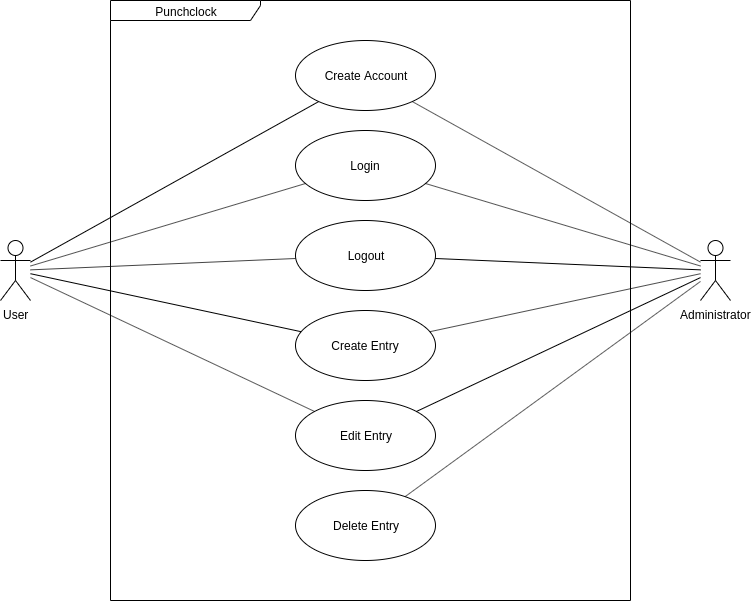
\includegraphics[width=\textwidth]{images/UseCaseDiagram.png}
        \caption{Use Case-Diagramm}
        \label{usecase}
    \end{figure}
    \subsection{Akteure}
    Benutzer können sich anmelden, abmelden und Entries verwalten.

    \subsection{Anforderungen}
    \subsubsection{Create Account}
    Neue Benutzer können einen eigenen Account erstellen. Dazu
    brauchen sie eine Email-Adresse und ein Passwort, welches
    den Anforderungen entsprechen.

    \subsubsection{Login}
    Bestehende Benutzer können sich anmelden. Dazu werden wiederum
    die Email-Adresse, welche sie zur Erstellung verwendet wurde,
    und das dazugehörige Passwort benötigt. Ein Aktivitätsdiagram
    dazu finden Sie in Abbildung \ref{activity}

    \begin{figure}
        \begin{center}
            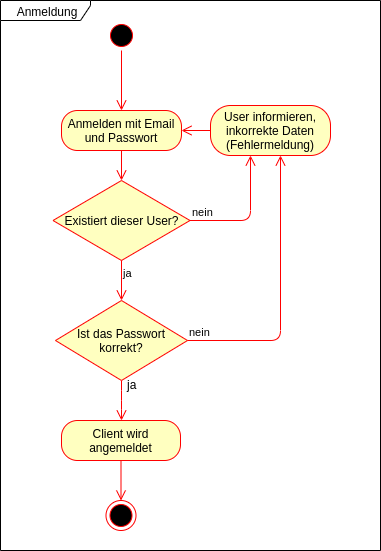
\includegraphics[width=6cm]{images/Aktivitaetsdiagramm.png}     
        \end{center}
        \caption{Aktivitätsdiagramm}
        \label{activity}
    \end{figure}

    \subsubsection{Logout}
    Eingeloggte Benutzer können sich wieder abmelden. Dazu müssen
    sie zunächst angemeldet sein.

    \subsubsection{Manage Entries}
    Eingeloggte Benutzer können neue Entries erstellen, lesen,
    bearbeiten und wieder löschen.

    \subsection{Nicht funktionale Anforderungen}
    \subsubsection{Performance}
    Die Datenbankabfragen müssen möglichst performant ablaufen, um die
    Userexperience nicht einzuschränken.
    \subsubsection{Design}
    Einheitliches Design in der Webapplikation, um die Userexperience zu
    optimieren.
    \subsubsection{Simple Authentifizierung}
    Die Applikation benötigt Authentifizierung. Die Tokens werden im
    Frontend gespeichert, sodass der Benutzer sich nicht jedesmal erneut
    einloggen muss. Für das Login werden lediglich Email und Passwort
    benötigt.
    \subsubsection{Sicherheit}
    Um die bestmögliche Sicherheit zu garantieren, wird HTTPS verwendet
    und ein ORM verwendet, um Database Injection zu vermeiden.

    \section{Datenhaltung}
    Die Applikation besteht aus vier Datenklassen (siehe Abbildung \ref{fachklassen}):
    \begin{itemize}
        \item ApplicationUser
        \item Entry
        \item Position
        \item Department
    \end{itemize}

    \begin{figure}
        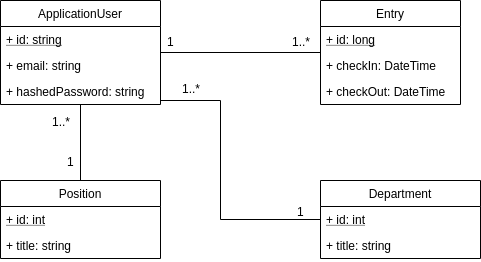
\includegraphics[width=\textwidth]{images/Fachklassendiagramm.png}
        \caption{Fachklassendiagram}
        \label{fachklassen}
    \end{figure}

    \section{Architektur}
    \subsection{Packagediagramm}
    Ich verwende sechs Namespaces, zwei für die Datenbank und vier für die
    GraphQL API (siehe Abbildung \ref{packages}).

    \begin{figure}
        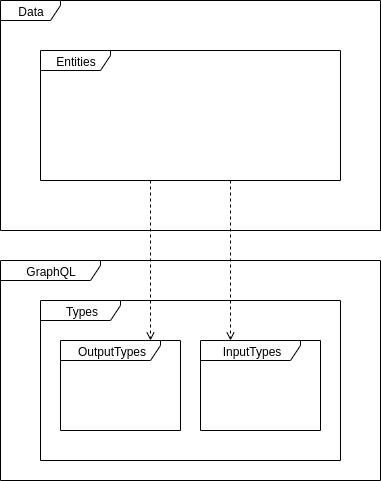
\includegraphics[width=\textwidth]{images/Packagediagramm.png}
        \caption{Packagediagramm}
        \label{packages}
    \end{figure}
    
    \subsection{Klassendiagramm}
    Ich verwende Klassen für die Datenbank-Entitäten und für die
    GraphQL Types. Ausserdem gibt es eine Startup-Klasse für die 
    Projektkonfiguration (siehe Abbildung \ref{classdiagram}).

    \begin{figure}
        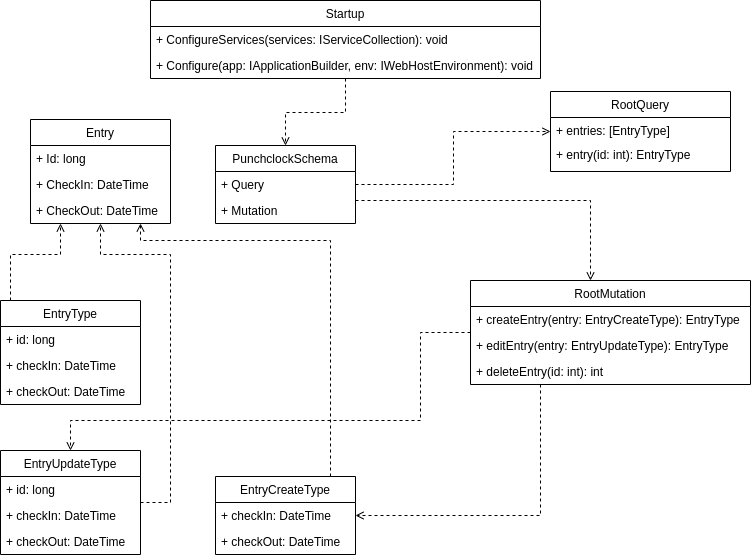
\includegraphics[width=\textwidth]{images/Klassendiagramm.png}
        \caption{Klassendiagramm}
        \label{classdiagram}
    \end{figure}

    \subsection{Deploymentdiagramm}
    Da wir lediglich auf localhost deployen, entstehen zwei Ports und eine
    Datenbank, welche als einfaches File eingesetzt wird. Auf Port 5001
    wird eine GraphQL Api mit .NET Core eingesetzt, auf Port 3000 entsteht
    eine React Applikation (siehe Abbildung \ref{deployment}).

    \begin{figure}
        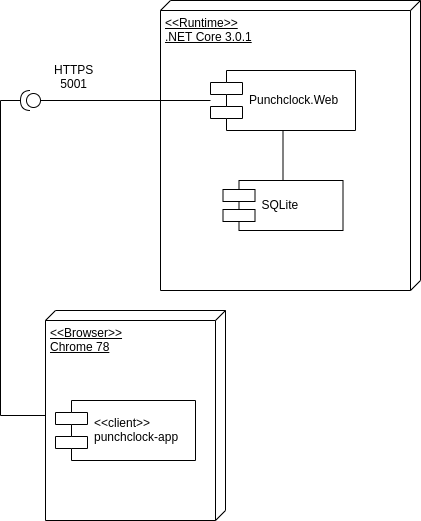
\includegraphics[width=\textwidth]{images/Deploymentdiagramm.png}
        \caption{Deploymentdiagramm}
        \label{deployment}
    \end{figure}

\end{document}